%%%%%%%%%%%%%%%%%%%%%%%%%%%%%%%%%%%%%%%%%%%%%%%%%%%%%
%			GENERÁTOR v. 18.09 				%
%%%%%%%%%%%%%%%%%%%%%%%%%%%%%%%%%%%%%%%%%%%%%%%%%%%%%
% Tento soubor slouží k jednotlivé zkusné kompilaci 
% písniček či k kompilaci samostatných pdf souborů 
% pomocí bashového skriptu kompilace.sh ve stejné 
% složce. Z důvodu hromadné kompilace musí poslední 
% dva řádky tohoto souboru zůstat nezměněny.
%%%%%%%%%%%%%%%%%%%%%%%%%%%%%%%%%%%%%%%%%%%%%%%%%%%%%
%			Jak kompilovat jednotlivé písně?        %
%%%%%%%%%%%%%%%%%%%%%%%%%%%%%%%%%%%%%%%%%%%%%%%%%%%%%
%	1. Do míst PÍSNIČKA upravte následnující řádek, 
%	   aby vypadal takto: 
%	   \input{../songy/[JMÉNO SOUBORU KOMPILOVNÉ PÍSNIČKY].tex}
%	2. Soubor písničky musí být přeložitelný a musí 
%	   se nacházet ve složce ../songy.
%%%%%%%%%%%%%%%%%%%%%%%%%%%%%%%%%%%%%%%%%%%%%%%%%%%%%
%			Jak psát soubory songů?                 %
%%%%%%%%%%%%%%%%%%%%%%%%%%%%%%%%%%%%%%%%%%%%%%%%%%%%%
%	1. Více návodu je k tomuto napsáno v souboru 
%      ../songy/00Songtemplate. 
%%%%%%%%%%%%%%%%%%%%%%%%%%%%%%%%%%%%%%%%%%%%%%%%%%%%%
%			Jak kompilovat celý zpěvník?			%
%%%%%%%%%%%%%%%%%%%%%%%%%%%%%%%%%%%%%%%%%%%%%%%%%%%%%
%	1. Více návodu je k tomuto napsáno v souboru
%	   ../Cely_zpevnik/zpevnik.tex.
%%%%%%%%%%%%%%%%%%%%%%%%%%%%%%%%%%%%%%%%%%%%%%%%%%%%%

% Hlavička START
\documentclass[openany,12pt]{memoir}
\usepackage[utf8]{inputenc} 
\usepackage[czech]{babel}
\usepackage[T1]{fontenc}
\usepackage[top=1.5cm, bottom=2cm, left=2cm, right=2cm]{geometry}  % --> NASTAVENÍ OKRAJŮ
\usepackage{fancyhdr}
\usepackage{graphicx}
\usepackage{xwatermark}
\usepackage{xcolor}
\usepackage{changepage}
\usepackage{pdfpages}
\usepackage{lettrine}
\usepackage{indentfirst}  %Důležité pro formátování

%%%%%%%%%%%%%%%%%%%%%%%%%%%%%%%%%%%%%%
%  FONT                              %
%%%%%%%%%%%%%%%%%%%%%%%%%%%%%%%%%%%%%%
\usepackage{amssymb}
\usepackage{tgschola}



%%%%%% Package na zpěvník
\usepackage[full]{leadsheets}%http://mirrors.nic.cz/tex-archive/macros/latex/contrib/leadsheets/leadsheets_en.pdf   --> dokumentace	
\definesongtitletemplate{empty}{} 
\setchords{
format = \bfseries \sffamily,   %tučné akordy
minor = {mi},% 
input-notation = {german},%
output-notation = {german}%
}
\definesongtitletemplate{empty}{} 


\newlength{\drop}
% VODOZNAK
\newwatermark[pages=1-,color=red!50,angle=0,scale=2, xpos=0,ypos=0]{
\includegraphics[width=5cm]{obr/pozadi2.jpg}} %--> dvojka na pozadí


%%%%%%%%%%%%%%%%%%%%%%%%%%%%%%%%%%%%%%%%%%%%%%%%%%
%		 Vlastní příkazy
\newcounter{Slokočet}   %Automatické číslování slok
\newcommand{\mezera}{
\phantom{.}

}   %Horizontální odsazení slok (poněkud blbě zadefinovaný, ale jinak se formát rozbije jako wtf prostě)
\newcommand{\stred}{5.2cm}   %%% Na zarovnání slok doprostřed, pozn. automatičtější zarovnávání na střed nejde
\newcommand{\carka}{,\:}
\newcommand{\m}[1]{\color{white}{#1}}  %Pro akordy
\newcommand{\ap}{'}	%Pro apostrof
\newcommand{\elipsa}{\kern\fontdimen3\font} %Příkaz pro lepší zacházení s výpustkami (=...); je to vpodstatě jen mezera mezi tečkama výpustky
\newcommand{\pindent}{17.62482 pt} %Správná velikost \parindentu u layoutu se dvěma minipageama
\newcommand{\predtitle}{\huge}
\newcommand{\mezisloupci}{\phantom{TT}} %Místo mezi dvěma sloupci na jedné stránce
\newcommand{\z}{\hspace*{\fill}\null}

%%% Možné velikosti písem 
\newcommand{\normalni}{\normalsize}
\newcommand{\velky}{\fontsize{14.4}{15}\selectfont}
\newcommand{\vetsi}{\fontsize{15}{16}\selectfont}
\newcommand{\nejvetsi}{\fontsize{16}{17}\selectfont}
\newcommand{\nejnejvetsi}{\fontsize{17}{19}\selectfont}

%%% Stará definice sloky spoléhající na indenty
%\newlength{\pismeno}
%\settowidth{\pismeno}{x} %Tohle není moc ideální velikost, ale funguje
%\newif\ifslokavelka
%\slokavelkafalse
%\newcommand{\sloka}{
%\ifnum \value{Slokočet}>8  %Pokud je sloka dvouciferná
%\mezera \noindent \addtocounter{Slokočet}{1} \hspace*{-\pismeno}\arabic{Slokočet}.
%\else %Pokud jen jednociferná
%\mezera \noindent \addtocounter{Slokočet}{1} \arabic{Slokočet}. 
%\fi
%} 	%sloka, která se automaticky čísluje

\newcommand{\distanc}{\:}  %Vzdálenost čísla sloky před slokou
\newlength{\delkaargumentu}
%%% Sloka s automatickým číslováním
\newcommand{\sloka}{%
\addtocounter{Slokočet}{1}% Zvýší se o 1 počet slok
\mezera%  Sloka se odsadí vertikálně
\settowidth{\delkaargumentu}{\arabic{Slokočet}.\distanc}% Zde se určí délka odsazení 
\hspace*{-\delkaargumentu}%
\arabic{Slokočet}.\distanc%
\ignorespaces% Aby nevznikaly zbytečné mezery
}


%%% Sloka s vlastním argumentem
\newcommand{\ssloka}[1]{%     
\settowidth{\delkaargumentu}{#1\distanc}
\mezera%
\hspace*{-\delkaargumentu}%
#1\distanc%
\ignorespaces%
}  

%%% Refrén
\newcommand{\refren}[1][0]{%  Nepovinný argument sděluje, kolikátý refrén toto je, bez argumentu se vytiskne pouze refrén
\ifnum #1>0 %Pokud nepovinný argument existuje
\mezera%
\settowidth{\delkaargumentu}{\textbf{R$_{\text{#1}}$:}\distanc}%
\hspace*{-\delkaargumentu}%
\textbf{R$_{\text{#1}}$:}\distanc%
\ignorespaces%
\else %Pokud nepovinný argument neexistuje
\mezera%
\settowidth{\delkaargumentu}{\textbf{R:}\distanc}%
\hspace*{-\delkaargumentu}%
\textbf{R:}\distanc%
\ignorespaces%
\fi
}

\newcommand{\predehra}{\ssloka{\textbf{Předehra:}}}

%%% Capo
\newcommand{\capo}[1]{%
\emph{Capo #1}
}


\addto\captionsczech{\renewcommand{\contentsname}{Seznam písní}}

%%%%%%%%%%%%%%%%%%%%%%%%%%%%%%%%%%%%
%    FORMÁTOVÁNÍ                   %
%%%%%%%%%%%%%%%%%%%%%%%%%%%%%%%%%%%%

%%% Vlevo zarovnaný text s blokem zarovnaným na střed
\usepackage{varwidth}% http://ctan.org/pkg/varwidth
\newenvironment{centerjustified}{%
  \begin{center} % so the minipage is centered
  \begin{varwidth}[t]{\textwidth}	
  \raggedright % so the minipage's text is left justified
  \setlength{\parindent}{\pindent}
}{%
  \end{varwidth}
  \end{center}
}


%Hlavnička END
\begin{document}
\sffamily %Sans-serif pro lepší čitelnost

\pagestyle{empty}
\newgeometry{top=1.5cm, bottom = 0cm, left = 2cm, right = 2cm}
	
\newpage

%Pro kompilaci je důležitý, aby ten \input a \end{document} zůstali na posledních
%dvou řádcích!!!!

\velky
\newpage
% PÍSNIČKA
\begin{song}{title=\predtitle \centering Wonderwall \\\large Oasis }  %% sem se napíše jméno songu a autor

\vspace*{.5cm}

\begin{centerjustified}
\vetsi


\kapodastr{2}

\predehra
$4\times$ \writechord{Emi7 G Dsus4 A7sus4}


\sloka
^{Emi7\z}Today is ^{G\z}gonna be the day

That they're ^{Dsus4\z}gonna throw it back ^{A7sus4}to~you.

^{Emi7\z}By~now you ^{G\z}should've somehow

^{Dsus4}Realised what you ^{\z A7sus4}gotta~do.


^{Emi7}I~don't believe that ^{G\z}anybody

^{\z Dsus4}Feels the ^*{A7sus4}way~I~do~abo ut you ^{Cadd9}now. ^{Dsus4 A7sus4}


\sloka
^{Emi7 \z}Backbeat the ^{G \z}word is on the street

That the ^{Dsus4 \,}fire in your heart ^{A7sus4 \z}is~out.

^{Emi7 \z}I'm~sure you've ^{G \z}heard it all before

But you ^{Dsus4}never really had ^{A7sus4 \z}a~doubt.

^{Emi7 \z}I~don't believe that ^{G \z}anybody ^{Dsus4}feels

The way I ^{A7sus4 \z}do~about you ^{Emi7}now. ^{G Dsus4 A7sus4}


\end{centerjustified}
\newpage
\begin{centerjustified}


\refren[1]
And ^{Cadd9 \z}all~the roads ^{Dsus4}we~have~to walk ^*{Emi7}are~w inding.

And ^{Cadd9 \z}all~the lights ^{\z Dsus4}that lead us there ^*{Emi7}are~bl inding.

^{Cadd9}There are many ^*{Dsus4}thing s that I would

^*{G\z}Li ke to ^{D/F# \z}say~to ^{Emi7}you

But ^*{G \z}I~don 't know ^{\z A7sus4}how.~~~

\vspace{-0.1cm}

\refren[2]
Because ^{Cadd9 \z}maybe ^{Emi7 G}

You're ^{Emi7 \z}gonna be the one that ^{Cadd9\z}saves me? ^{Emi7 G}

And ^{Emi7}after ^{Cadd9 \z}all~~~~~~ ^{Emi7 G}

You're ^{Emi7}my ^{\z Cadd7}wonderwall.~~~~ ^{Emi7 G Emi7(Break)}

\vspace{-0.1cm}

\sloka
Today was gonna be the day

But they'll never throw it back to you.

By now you should've somehow

Realised what you're not to do.

I don't believe that anybody

Feels the way I do

About you ^{Cadd9}now.~ ^{Dsus4 A7sus4}

\vspace{-0.1cm}

\refren[1]

\vspace{-0.1cm}

\refren[2]
I said maybe \dots

\refren[2]
I said maybe (I said maybe) \dots

\phantom{.}

I said maybe. (I said maybe)

/: You're ^{Emi7}gonna be the one that ^{Cadd9\z}saves me? (that ^{Emi7 \z}saves ^{\z G}me) :/

You're gonna be the one that saves me? (that saves me)

\ssloka{\textbf{Sólo:}}\\
\vspace{-0.3cm}
\centering
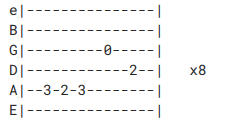
\includegraphics[scale=3]{../taby/wonderwall.png}

\vspace{.5cm}
% 
\includegraphics[width=3cm]{../Akordy/a7sus4.png} % akordy se tu hraji celkove jinak, tak ze se dohromady lepe prehmatavaji -> tzn toto by tu bylo matouci
\end{centerjustified}
\setcounter{Slokočet}{0}
\end{song}

\end{document}
